\section{Removing the ratio condition: unconditional theorems}
\label{sec:removing}

\subsection{What has to be shown}

Corollary~\ref{cor:regular} needs a bound on $\Lambda = 4\xb(\sqrt\varrho)$ itself. Theorem~\ref{thm:log} obtained one through $\xb(\varrho)$ and the ratio $K_\Lambda$. A direct route needs only the following form, in which the information along the stable direction plays the role of the scale.

\begin{proposition}[Target inequality]
\label{prop:target}
Suppose that $\Lambda \leq A + B\ln\big(1/(\sigma^2 J_{ww})\big)$ for a state satisfying (H2). Then
\begin{gather}
g \geq \Pi\,\frac{c}{\sqrt{\ln(1/\sigma) + C}}, \qquad c = \frac{1}{\pi\sqrt B}, \label{eq:target}\\
C = \frac12\ln\big(2(\pi^2 + \sigma^2)\big) + \frac{A}{2B}. \nonumber
\end{gather}
\end{proposition}

\begin{proof}
Insert Eq.~\eqref{eq:CR} into the hypothesis and the result into Corollary~\ref{cor:regular}.
\end{proof}

By Lemma~\ref{lem:fisher}(b) below, $\Lambda \leq 2 + 8tR$, where $tR$ is the rate at which the information along the stable direction is lost under further blurring (Eq.~\eqref{eq:Rdef}). The theorems below prove the hypothesis of Proposition~\ref{prop:target} for their classes in the stronger form
\begin{equation}
tR \leq A' + B'\ln\frac{1}{tJ_{ww}},
\label{eq:T2}
\end{equation}
which gives $B = 8B'$ and $A = 2 + 8A'$. For general states we conjecture the law itself:

\begin{conjecture}[Logarithmic law for all states]
\label{conj:general}
There are constants $c > 0$ and $C$ such that every state satisfying (H1) and (H2) obeys $g \geq \Pi\,c/\sqrt{\ln(1/\sigma) + C}$.
\end{conjecture}

We state the conjecture for the gap rather than for Eq.~\eqref{eq:T2}, because Eq.~\eqref{eq:T2} with universal constants is not true for every state. In work to be reported separately we find states in which hidden sources of alternating sign sit in a deep valley between long lines along $w$; for them $tR/\ln(1/(tJ_{ww}))$ grows without bound as the number of sources grows (numerical results and a leading-order analysis). Such states need lines whose length is exponential in the depth of the valley, so (H2) limits the effect, and they do not by themselves contradict Conjecture~\ref{conj:general}.

\subsection{The Fisher form and the heat flow}

Write $t$ for the blur variance and follow the state along the heat flow $\partial_t\varrho = \frac12\Delta\varrho$, which is the blur growing from $t = 0$ to $t = \sigma^2$. Define the rate at which the information along the stable direction is lost,
\begin{equation}
R(t) = -\frac{d\ln J_{ww}}{dt} .
\label{eq:Rdef}
\end{equation}

\begin{lemma}[Fisher form]
\label{lem:fisher}
For every state, (a)~$\Lambda \leq 2 + 8t\,\E[H_{vw}^2]/J_{ww}$; (b)~$dJ_{ww}/dt = -\E[H_{vw}^2 + H_{ww}^2]$, so that $tR = t\,\E[H_{vw}^2 + H_{ww}^2]/J_{ww}$ and $\Lambda \leq 2 + 8tR$; (c)~with $u = s_w$ and $L = \Delta + s\cdot\nabla$,
\begin{equation}
J_{ww}R' = -\E[(Lu + Ru)^2] - \E[(H^3)_{ww}] .
\label{eq:gamma2}
\end{equation}
\end{lemma}

Part (a) follows from two integrations by parts and the bound $H_{vv} \leq 1/t$, which holds because the posterior covariance $t I - t^2 H$ is positive semidefinite; (b) is a directional de~Bruijn identity; (c) is the Bochner, or $\Gamma_2$, identity of the operator $L$~\cite{bakry2014} applied to $u$. The proofs are in Appendix~\ref{app:fisher}. The first term of Eq.~\eqref{eq:gamma2} is never positive. The second can be positive only where $H$ has a negative eigenvalue, that is, where the blurred density is log-convex in some direction: in the valleys between peaks. In particular, for a log-concave state $H \succeq 0$, so $R$ never increases and $J_{ww}$ is log-convex along the heat flow, a directional counterpart of the concavity of $1/I$ along the heat flow for log-concave densities~\cite{toscani2015}. For multimodal states $R$ can increase; for two clusters we found $R(\sigma^2/4)/R(\sigma^2) = 0.70$.

The heat flow converts a bound on the growth of $R$ into the target inequality.

\begin{lemma}[Integration along the heat flow]
\label{lem:integration}
If $t^2R'(t) \leq A_1\,tR(t) + \kappa_1$ for all $t \in [\tau\sigma^2, \sigma^2]$, with constants $A_1, \kappa_1 \geq 0$ and $\tau \in (0,1)$, then
\begin{equation}
\Lambda \leq 2 + 8c_0 + B\Big[\ln\frac1\tau + \ln\frac{1}{\sigma^2 J_{ww}}\Big], \qquad B = \frac{8(1 + A_1)}{1 - \tau^{1+A_1}},
\end{equation}
with $c_0 = \kappa_1\big[\ln(1/\tau)/(1 - \tau^{1+A_1}) - 1/(1 + A_1)\big]$.
\end{lemma}

\begin{proof}
The hypothesis gives $d(s^{-A_1}R)/ds \leq \kappa_1 s^{-A_1-2}$, so that $R(s) \geq (s/\sigma^2)^{A_1}R(\sigma^2) - \kappa_1\big(1/s - s^{A_1}/\sigma^{2+2A_1}\big)/(1+A_1)$ for $s \leq \sigma^2$. Integrating over $[\tau\sigma^2, \sigma^2]$ and using $\int R = \ln\big(J_{ww}(\tau\sigma^2)/J_{ww}(\sigma^2)\big)$ and $J_{ww}(\tau\sigma^2) \leq 1/(\tau\sigma^2)$, the Fisher information of a blur of variance $\tau\sigma^2$, bounds $\sigma^2 R(\sigma^2)$. Lemma~\ref{lem:fisher}(b) then bounds $\Lambda$.
\end{proof}

So the question becomes whether the valleys, the only source of growth of $R$ in Eq.~\eqref{eq:gamma2}, can be controlled.

\subsection{Deep valleys cost Fisher information}

On a line, the blurred density is the Gaussian blur of a positive measure. Let $c(y)$ be the posterior variance at $y$ in units of $t$, so that $c - 1 = -t\,\partial^2\ln\varrho$; a valley is a point with $c > 1$, and a deep valley one with $c \geq 1 + \eta$. In units $t = 1$:

\begin{lemma}[A valley is a dip]
\label{lem:dip}
$\ln\varrho(y+u) + \ln\varrho(y-u) - 2\ln\varrho(y) \geq \ln\cosh\big(u\sqrt{2c(y)}\big) - u^2$ for all $u$.
\end{lemma}

\begin{proof}
$\varrho(y\pm u) = \varrho(y)e^{-u^2/2}\E_y[e^{\pm u(X - y)}]$, with $\E_y$ the posterior at $y$. The product of the two is $\varrho(y)^2e^{-u^2}\E[\cosh(u(X - X'))]$ for two independent posterior copies, and $x \mapsto \cosh(u\sqrt x)$ is convex, so Jensen's inequality gives $\E[\cosh(u|X - X'|)] \geq \cosh(u\sqrt{2c})$.
\end{proof}

For $c$ well above one the right side is positive: the valley point lies at the bottom of a dip of depth about $u\sqrt{2c} - u^2$. Climbing out of a dip requires score. If $\varrho(b) \geq \varrho(a)e^{\Delta}$ with $\Delta \geq 0$, then $\int_a^b \varrho\,s^2 = 4\int_a^b (\sqrt\varrho\,')^2 \geq 4\varrho(a)(e^{\Delta/2} - 1)^2/(b - a)$ by the Cauchy--Schwarz inequality. Applying this on both sides of the dip, with the convexity of $x \mapsto (e^{x/2}-1)_+^2$, gives $\varrho(y) \leq u\big(8(e^{D/4} - 1)^2\big)^{-1}\int_{|y'-y| \leq u}\varrho\,s^2$, where $D$ is the right side of Lemma~\ref{lem:dip}. Integrating over the valley points, exchanging the integrals and choosing $u$ for each range of $c$ gives:

\begin{theorem}[Valleys cost Fisher information]
\label{thm:valley}
For every state on a line and every $\eta > 0$,
\begin{equation}
\E\big[(c - 1)^3\,\mathbf{1}\{c \geq 1 + \eta\}\big] \leq \kappa_\eta\, t J,
\end{equation}
where $J$ is the Fisher information and $\kappa_\eta$ is an explicit constant; $\kappa_{0.1} = 267$.
\end{theorem}

The constant is loose: the largest value of the left side divided by $tJ$ that we found is about $3$. In observer language: where the observer is very unsure from which part of the state a point came, the density has a dip, and the slopes of the dip are score, that is, information.

\begin{theorem}[Product states]
\label{thm:product}
Let $\rho(x) = \rho_1(f\cdot x)\rho_2(l\cdot x)$ for an orthonormal pair $(f, l)$ at any angle, including states concentrated on a line, and let (H2) hold. Then $t^2R' \leq \eta\,tR + \kappa_\eta$ for every $t$ and $\eta > 0$, and the logarithmic law~\eqref{eq:target} holds without any ratio condition, with $B = 8(1+\eta)/(1-\tau^{1+\eta})$ for any $\tau \in (0,1)$. For $\eta = 0.1$ and $\tau = 1/4$, $c = 0.0949$ and $C = 84$ ($\sigma \leq 1$).
\end{theorem}

\begin{proof}
The blur preserves the product form, and $H$ is diagonal in $(f, l)$. With $a = (e_w\cdot f)^2$, $-(tH)^3_{ww} = a(c_f - 1)^3 + (1-a)(c_l - 1)^3$ and $J_{ww} = aJ_{ff} + (1-a)J_{ll}$, where $c_f$, $c_l$ are the posterior variances of the two factors. The part with $c < 1 + \eta$ is at most $\eta\,(tH)^2_{ww}$, and Theorem~\ref{thm:valley} for each factor bounds the rest by $\kappa_\eta tJ_{ww}$. Dropping the first term of Eq.~\eqref{eq:gamma2} gives $t^2R' \leq \E[-(tH)^3_{ww}]/(tJ_{ww}) \leq \eta\,tR + \kappa_\eta$. Lemma~\ref{lem:integration} and Proposition~\ref{prop:target} complete the proof.
\end{proof}

The large $C$ reflects only the loose $\kappa_\eta$; the coefficient $c$ does not depend on it.

\subsection{States without deep valleys, and the strips}
\label{sec:novalley}

In the plane the same mechanism works whenever the valleys stay shallow.

\begin{proposition}[No deep valleys]
\label{prop:novalley}
Suppose that (H2) holds and that for some $\tau \in (0,1)$ and $\Lambda_* \geq 0$ the posterior covariance satisfies $\Cov(X\mid y) \preceq (1 + \Lambda_*)\,t\,I$ for every $y$ and every blur $t \in [\tau\sigma^2, \sigma^2]$. Then $t^2R' \leq \Lambda_*\,tR$ on that window, and the logarithmic law~\eqref{eq:target} holds with $B = 8(1+\Lambda_*)/(1 - \tau^{1+\Lambda_*})$ and $A = 2 + B\ln(1/\tau)$.
\end{proposition}

\begin{proof}
The hypothesis says that every eigenvalue $\lambda_i$ of $-tH$ is at most $\Lambda_*$. With $a_i = (e_w\cdot f_i)^2$ for the eigenvectors $f_i$, $-(tH)^3_{ww} = \sum_i\lambda_i^3 a_i \leq \Lambda_*\sum_i\lambda_i^2a_i = \Lambda_*(tH)^2_{ww}$, since the terms with $\lambda_i \leq 0$ are not positive. Equation~\eqref{eq:gamma2} gives $t^2R' \leq \Lambda_*\,tR$, and Lemma~\ref{lem:integration} with $\kappa_1 = 0$ and Proposition~\ref{prop:target} complete the proof.
\end{proof}

\begin{observation}
\label{obs:novalley}
On the eight strip optima of Table~\ref{tab:gmin}, the largest eigenvalue of $-tH$ over all points and over 25 blurs $t \in [\sigma^2/4, \sigma^2]$ is $\Lambda_* = 1.8745$, at $\sigma = 10^{-2}$ and $t = \sigma^2/4$ (Fig.~\ref{fig:valleys}a). It decreases with $t$ on every strip, and its maximum over the window falls from $1.87$ at $\sigma = 10^{-2}$ to $0.38$ at $10^{-48}$ and $0.03$ at $10^{-96}$. Proposition~\ref{prop:novalley} then gives $c = 0.0658$ and $C = 2.28$ for the strips ($\tau = 1/4$, $\sigma \leq 1$).
\end{observation}

The values at $\sigma = 10^{-2}$ ($1.874$, $1.756$ and $1.537$ at $t = \sigma^2/4$, $\sigma^2/2$ and $\sigma^2$) were reproduced by an independent evaluation on a two-dimensional Fourier grid. The verification is a dense-grid evaluation, not interval arithmetic. In observer language, the strips never make the observer much more unsure than the blur itself: their fineness consists of shallow ripples, not valleys. On the strips Theorem~\ref{thm:log} with $K_1 = 1$ also applies, with a better constant (Fig.~\ref{fig:staircase}). The point of Proposition~\ref{prop:novalley} is that its hypothesis concerns valleys, the mechanism that Eq.~\eqref{eq:gamma2} identifies, rather than a ratio of norms.

\begin{figure}[t]
\centering
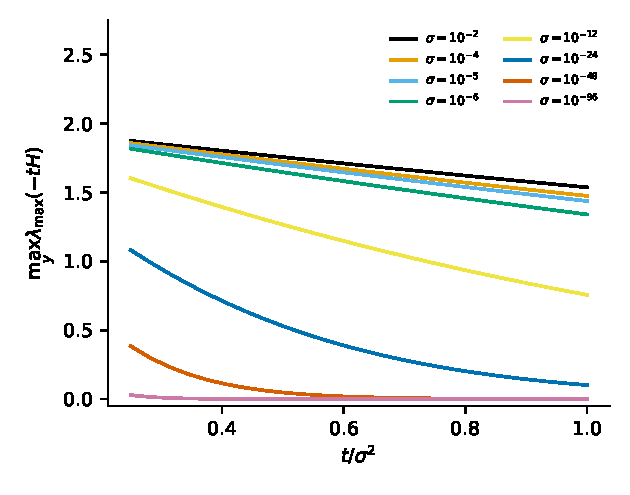
\includegraphics[width=0.95\columnwidth]{figures/fig5_valleys.pdf}
\caption{The strips have no deep valleys: largest eigenvalue of $-tH$ over all points, against the blur $t$ in the window of Proposition~\ref{prop:novalley}, for the eight strip optima. The values stay below $1.88$ and fall towards zero as $\sigma$ decreases.}
\label{fig:valleys}
\end{figure}

\subsection{What is now unconditional}

Putting the pieces together, the logarithmic law~\eqref{eq:target} holds with no ratio condition, under (H2) alone, for
\begin{itemize}
\item every product state $\rho_1(f\cdot x)\rho_2(l\cdot x)$, at any angle, including states concentrated on a line (Theorem~\ref{thm:product});
\item every state whose posterior covariance stays below $(1+\Lambda_*)$ times the blur on the window $[\tau\sigma^2, \sigma^2]$ (Proposition~\ref{prop:novalley}); the strips, the states that realise the smallest gaps we found, are in this class with $\Lambda_* = 1.87$ (Numerical result~\ref{obs:novalley}).
\end{itemize}
In both cases the mechanism is the same, and it is the one the observer would guess. Fine structure is what lets a state come close to $\kappa$, and the blur takes it away exponentially. The only way the blur can strip information faster is through valleys, places where the observer cannot tell from which part of the state a point came; and a valley is a dip whose slopes are paid for in information. The strips, which come closest to the edge, never pay that price: their fineness is all in shallow ripples.

What remains is Conjecture~\ref{conj:general} for states that do have deep valleys. Following the blur as it grows, the route used here, is not enough for every such state, and the confinement (H2) has to enter the argument (Sec.~\ref{sec:discussion}).
